\documentclass[conference,onecolumn,letterpaper,romanappendices,12pt,english,nofonttune]{IEEEtran}
    \IEEEoverridecommandlockouts
\usepackage[margin=1in]{geometry}
\usepackage{setspace}
\usepackage{tablefootnote}
\usepackage[compact]{titlesec}
\usepackage{float}
    \titlespacing{\title}{0pt}{0pt}{24pt}
    \titlespacing{\section}{0pt}{10pt}{6pt}
    \titlespacing{\subsection}{0pt}{*0}{*0}
    \titlespacing{\subsubsection}{0pt}{*0}{*0}
    \titlespacing{\appendix}{0pt}{*0}{*0}
    

\renewcommand{\appendix}{}

\usepackage[runin]{abstract}
    \renewcommand{\abstractnamefont}{\normalfont\normalsize\itshape}
    \renewcommand{\abstracttextfont}{\normalfont\normalsize}
    \setlength{\absleftindent}{0mm}
    \setlength{\absrightindent}{0mm}
    \abslabeldelim{--}

\usepackage{lastpage}
\usepackage{fancyhdr}
    \setlength{\headheight}{0.6in}
    \setlength{\headsep}{15pt}
    \setlength{\voffset}{-0.5in}
    \renewcommand{\headrulewidth}{0pt} % remove lines as well
    \renewcommand{\footrulewidth}{0pt}
    \fancyhf{}
    \fancyfoot[C]{\thepage\ of \pageref{LastPage}}
    \pagestyle{fancy}
   
\usepackage[ngerman,main=english]{babel}
\usepackage{xcolor}
\usepackage[pdftex]{graphicx}
\usepackage{wrapfig}
\usepackage{newtxtext,newtxmath}
\usepackage[group-minimum-digits=4,per-mode=fraction]{siunitx}
\usepackage[T1]{fontenc}
\usepackage{caption}
	\captionsetup[table]{labelsep=period,font=small,font=sc}
	\captionsetup[figure]{font=small,justification=centerlast}
\usepackage{subcaption}
\usepackage{booktabs}

\usepackage{enumitem}
\usepackage{soul}
\usepackage[noadjust]{cite}
    
\usepackage[capitalize,noabbrev]{cleveref}
    \crefname{figure}{Fig.}{Figs.}
    \crefname{equation}{}{}
    \crefname{section}{Section}{Sections}
    \crefname{table}{Table}{Tables}

\usepackage{multirow}

\renewcommand{\IEEEbibitemsep}{6pt}
\makeatletter
\IEEEtriggercmd{\reset@font\normalfont\fontsize{12pt}{12pt}\selectfont}
\makeatother
\IEEEtriggeratref{1}

%---folder for graphics and plots
\graphicspath{{./figures/}}

\hyphenation{op-tical net-works semi-conduc-tor}

 
\begin{document}
    \bstctlcite{bstctl:etal, bstctl:nodash, bstctl:simpurl}

\title{Real-Time Cyber Attack Detection Using IoT-Based Electric Measurement Units at the Point of Common Coupling (PCC)}
% \author{}
\maketitle

\begin{abstract}
As components of the electrical grid become increasingly connected through the internet, they face a growing threat from cyber attacks. This project developed a deep learning framework to detect anomalies in a multi-motor electrical motor testbed using features gathered by an EMU. EMUs are plug-and-play sensor devices placed at the Point of Common Coupling (PCC) that feed electrical motors in the testbed. EMUs produce data similar to micro-PMUs but are much cheaper, modular, and enable real-time data analysis through IoT compatibility. While initial baselines utilized standard Long Short-Term Memory (LSTM) networks, we ultimately developed a robust framework based on a Bidirectional Gated Recurrent Unit (GRU) architecture to better capture complex irregularities in time-series data. By addressing severe class imbalance and preserving raw signal context alongside temporal velocities, the proposed Bidirectional GRU model successfully transitioned from underfitting to strong generalization, achieving a testing accuracy of approximately 92\%.
\end{abstract}

\section{Introduction}
The integration of Internet of Things (IoT) technologies into the modern electrical grid has fundamentally transformed power distribution, enabling advanced monitoring, automation, and control at the consumer edge. However, this increased connectivity has concurrently expanded the attack surface for malicious cyber threats, such as False Data Injection Attacks (FDIAs)—implemented as ADC-offset bias on phase-current feedback—and distributed denial-of-service disruptions. Because cyber attacks on power systems rarely manifest as obvious, single-point physical failures—but rather as subtle, sequential deviations in electrical waveforms over time—standard static detection methods frequently fail to identify them, creating a critical need for advanced, time-series anomaly detection frameworks.

Traditional grid monitoring systems heavily rely on Phasor Measurement Units (PMUs) and micro-PMUs for high-fidelity anomaly detection. While these devices offer exceptional synchronization and monitoring capabilities, their reliance on high sampling frequencies and precise GPS synchronization makes them prohibitively expensive for widespread, ubiquitous deployment. This cost barrier results in limited deployment at the consumer edge, creating a significant visibility gap in the power distribution network where edge devices remain highly vulnerable to undetected intrusions.

To address this critical visibility gap, this work proposes the utilization of low-cost Electric Measurement Units (EMUs) as a scalable sensing platform. In our setup, EMUs (smart-plug form factor) are deployed at the point of common coupling (PCC) of a cyber-physical motor-drive testbed to emulate edge deployment conditions. The EMUs capture high-granularity AC power measurements with built-in IoT connectivity, enabling real-time edge analysis. We hypothesize that outlet-level EMU measurements contain sufficient feature richness to identify cyber anomalies without the financial overhead of micro-PMUs.

This digest presents a demonstration and rigorous benchmark of a supervised deep learning framework utilizing a Bidirectional Gated Recurrent Unit (GRU) network to detect cyber attacks from real-time EMU data streams. To handle the severe operational class imbalances inherent to authentic grid data, the framework integrates dynamic class weighting alongside custom precision-recall threshold tuning. By combining these training optimizations with a dual-stream feature engineering pipeline that preserves both raw signal magnitudes and temporal velocities, the proposed Bidirectional GRU framework successfully mitigates majority-class underfitting, achieving a robust testing accuracy of approximately 92\%.

The growing vulnerability of cyber-physical power systems to malicious intrusions has driven extensive research into advanced, real-time anomaly detection frameworks. Recent advancements have explored deep learning techniques for intrusion detection and mitigation at the device level. For example, Aljohani et al. \cite{aljohani2024} proposed an Intrusion Detection and Mitigation System (IDMS) utilizing Deep Learning Neural Networks (DLNNs) and Long Short-Term Memory (LSTM) networks to detect False Data Injection Attacks (FDIAs) targeting Intelligent Electronic Devices (IEDs). However, a primary limitation of this framework is its design focus on digitalized substations, which prevents it from providing ubiquitous, low-cost visibility at the consumer edge.

Furthermore, contemporary research has heavily focused on leveraging deep learning alongside Phasor Measurement Units (PMUs) for high-fidelity anomaly detection. Guha et al. \cite{guha} developed an LSTM-based Variational Autoencoder (VAE) to detect anomalies in unsupervised power grid data; yet, such approaches often assume relatively balanced operational states or require massive amounts of uncorrupted data, struggling with the severe class imbalances found in authentic grid environments. Similarly, recent evaluations of hybrid architectures, such as CNN-LSTMs \cite{pmu_lstm_2025}, have demonstrated high efficacy in detecting multi-class anomalies using PMU data streams. While highly effective, these existing methodologies are fundamentally limited by their reliance on the high sampling frequencies and precise GPS synchronization inherent to costly PMU monitoring equipment. 

Motivated by the cost/scalability limits of PMU/IED-centric methods, we present an EMU-based PCC solution; the key contributions are:
\begin{itemize}
    \item \textbf{Low-cost EMU-based PCC cyber-attack detection:} Real-time FDIA detection using IoT-enabled EMU measurements at the PCC as a scalable alternative to micro-PMUs.
    \item \textbf{Hybrid deep model + training pipeline for imbalanced time-series:} 1D-CNN + Bi-GRU with dual-stream (raw + temporal-differential) features and class-weighted training with PR-based threshold tuning, achieving a ~92\% test accuracy.
\end{itemize}

\section{Testbed Design and Dataset Structure}

\subsection{Testbed Design and Cyber-Attack Generation}
As illustrated in Fig.~\ref{fig:power_flow}, experiments are conducted on a cyber-physical motor-drive testbed consisting of an AC induction motor (ACIM)  and a permanent magnet synchronous motor (PMSM). To emulate consumer-edge monitoring, measurements are collected at the point of common coupling (PCC), where current and voltage sensors capture the aggregated electrical interaction of the drives. 
While PCC sensing is the focus of this study, stator current and voltage data at the motor-level are also available in the dataset for auxiliary monitoring and validation, and can be shared upon request for interested researchers.

\begin{figure}[H]
    \centering
    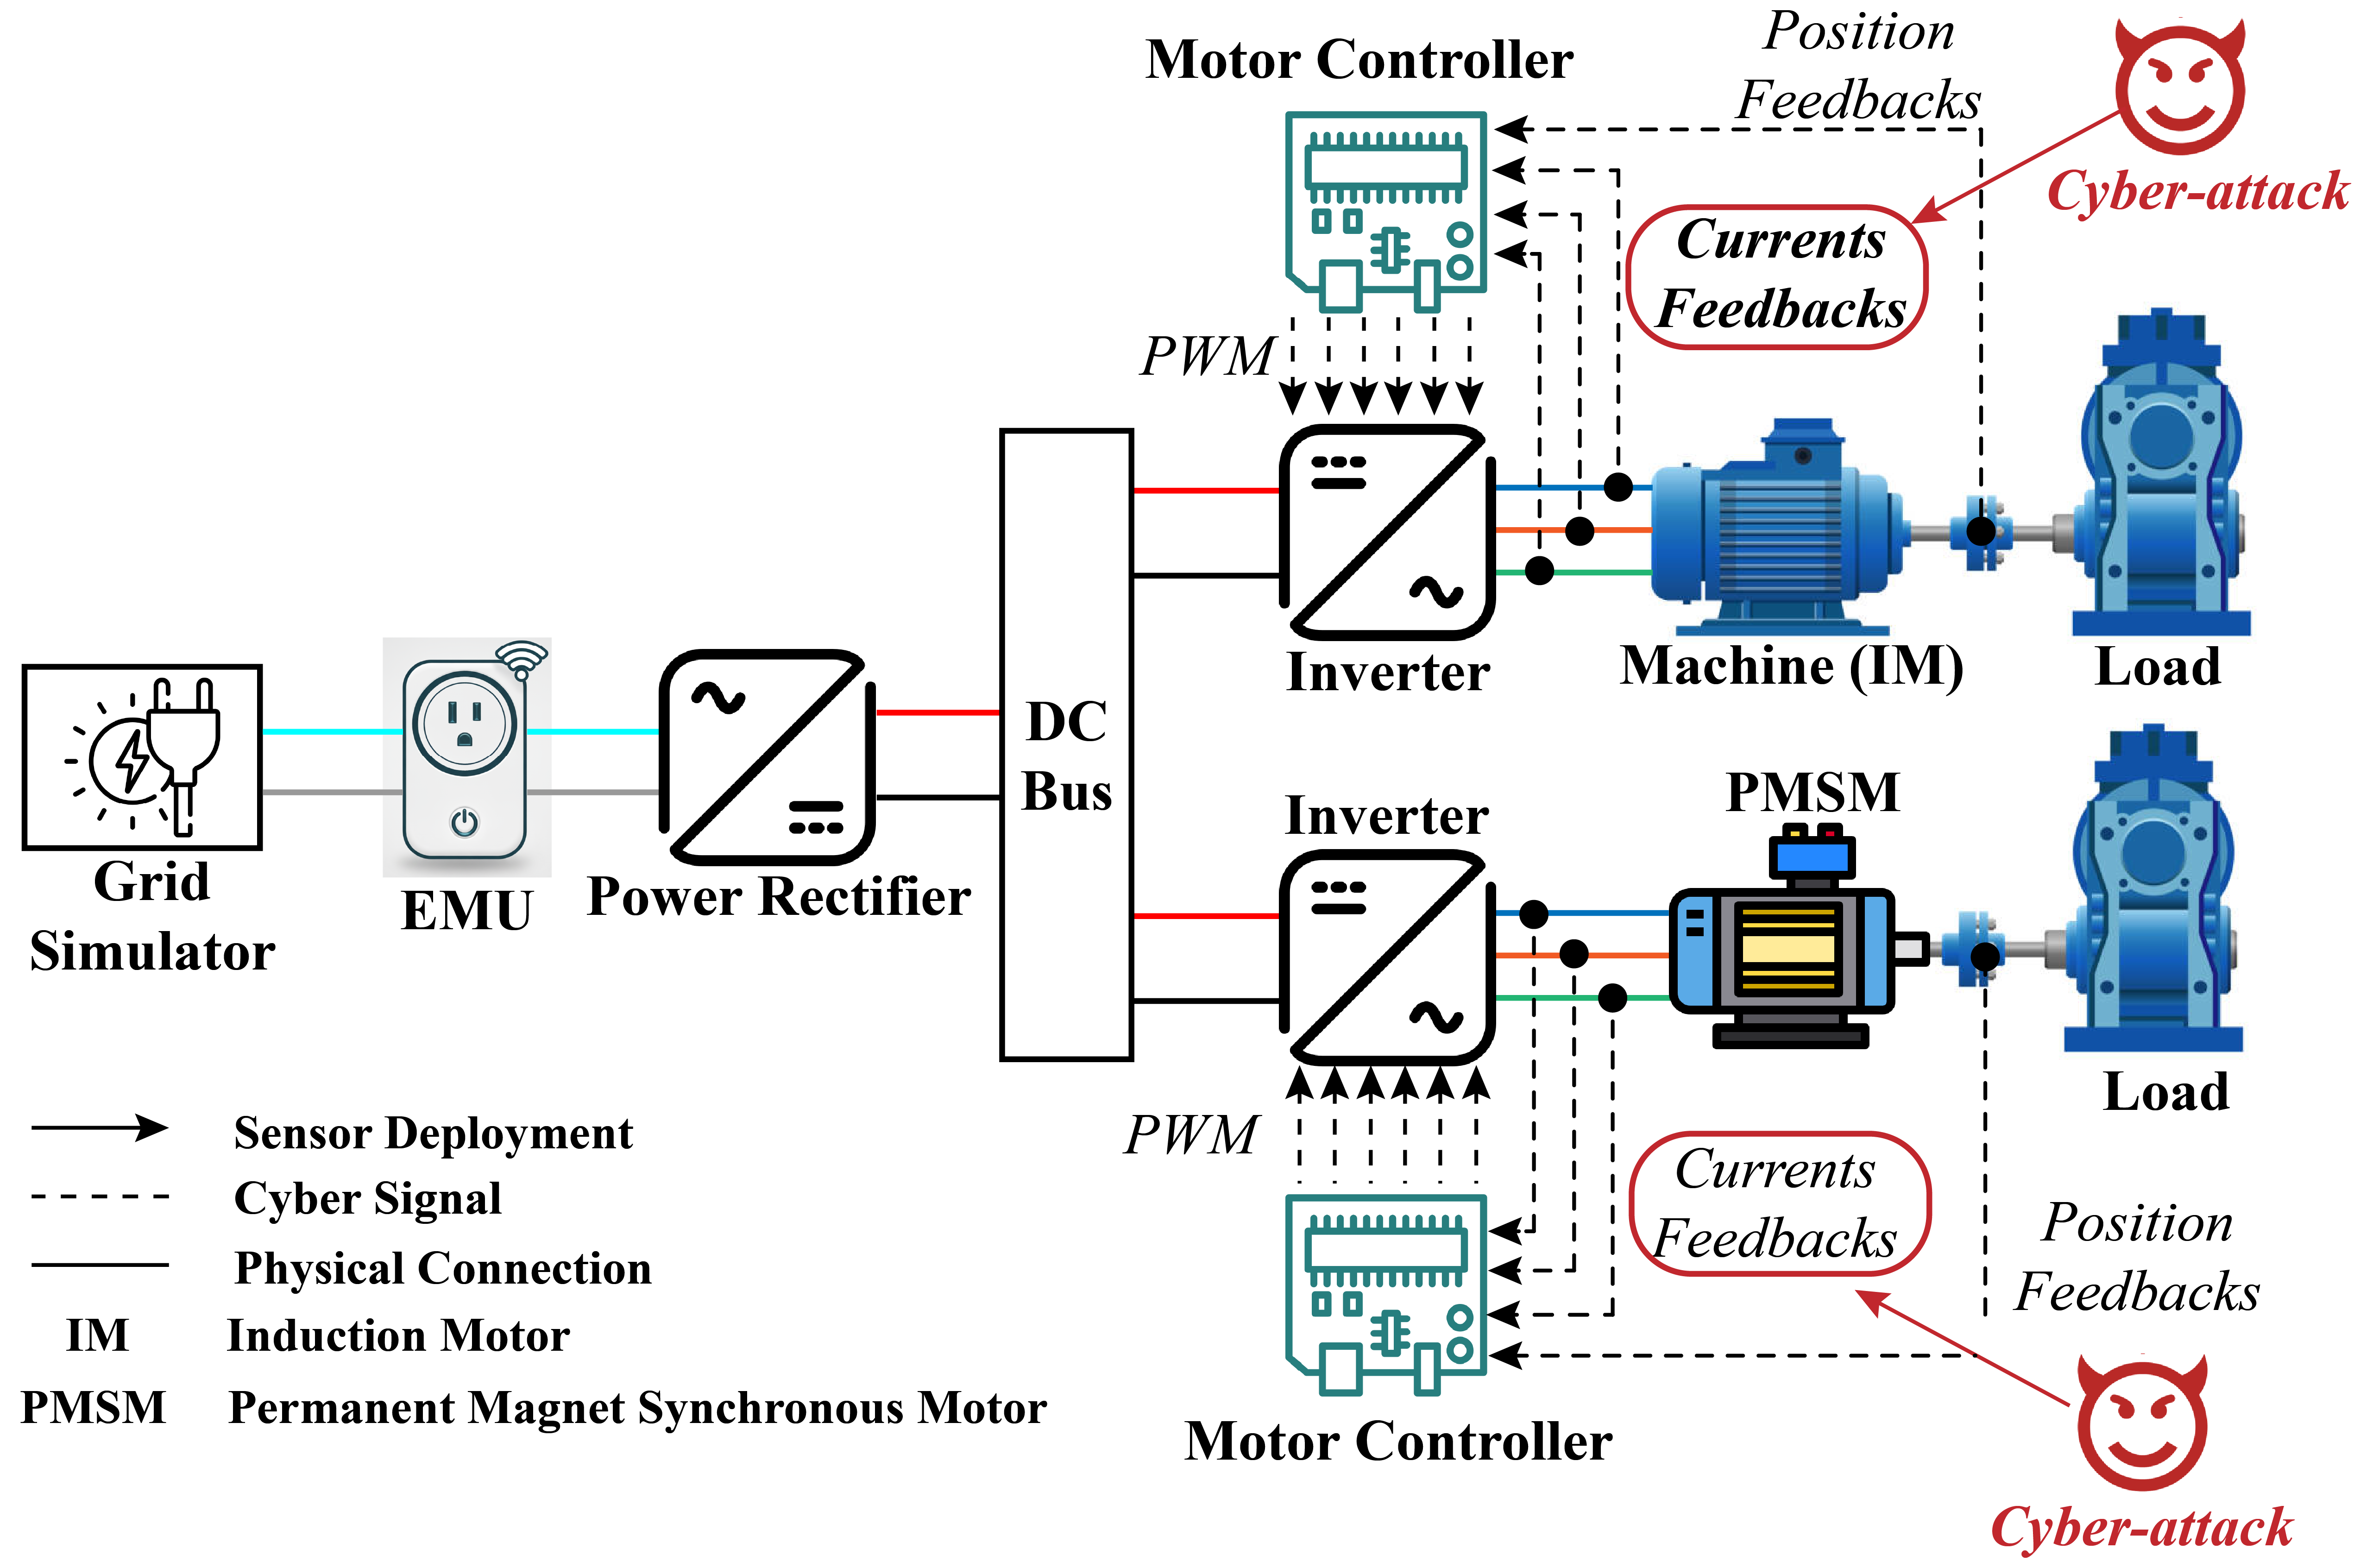
\includegraphics[width=0.6\linewidth]{figures/schematic diagram[18].png}
    \caption{Power Flow Schematic}
    \label{fig:power_flow}
\end{figure}
\begin{figure}[htpb]
    \centering
    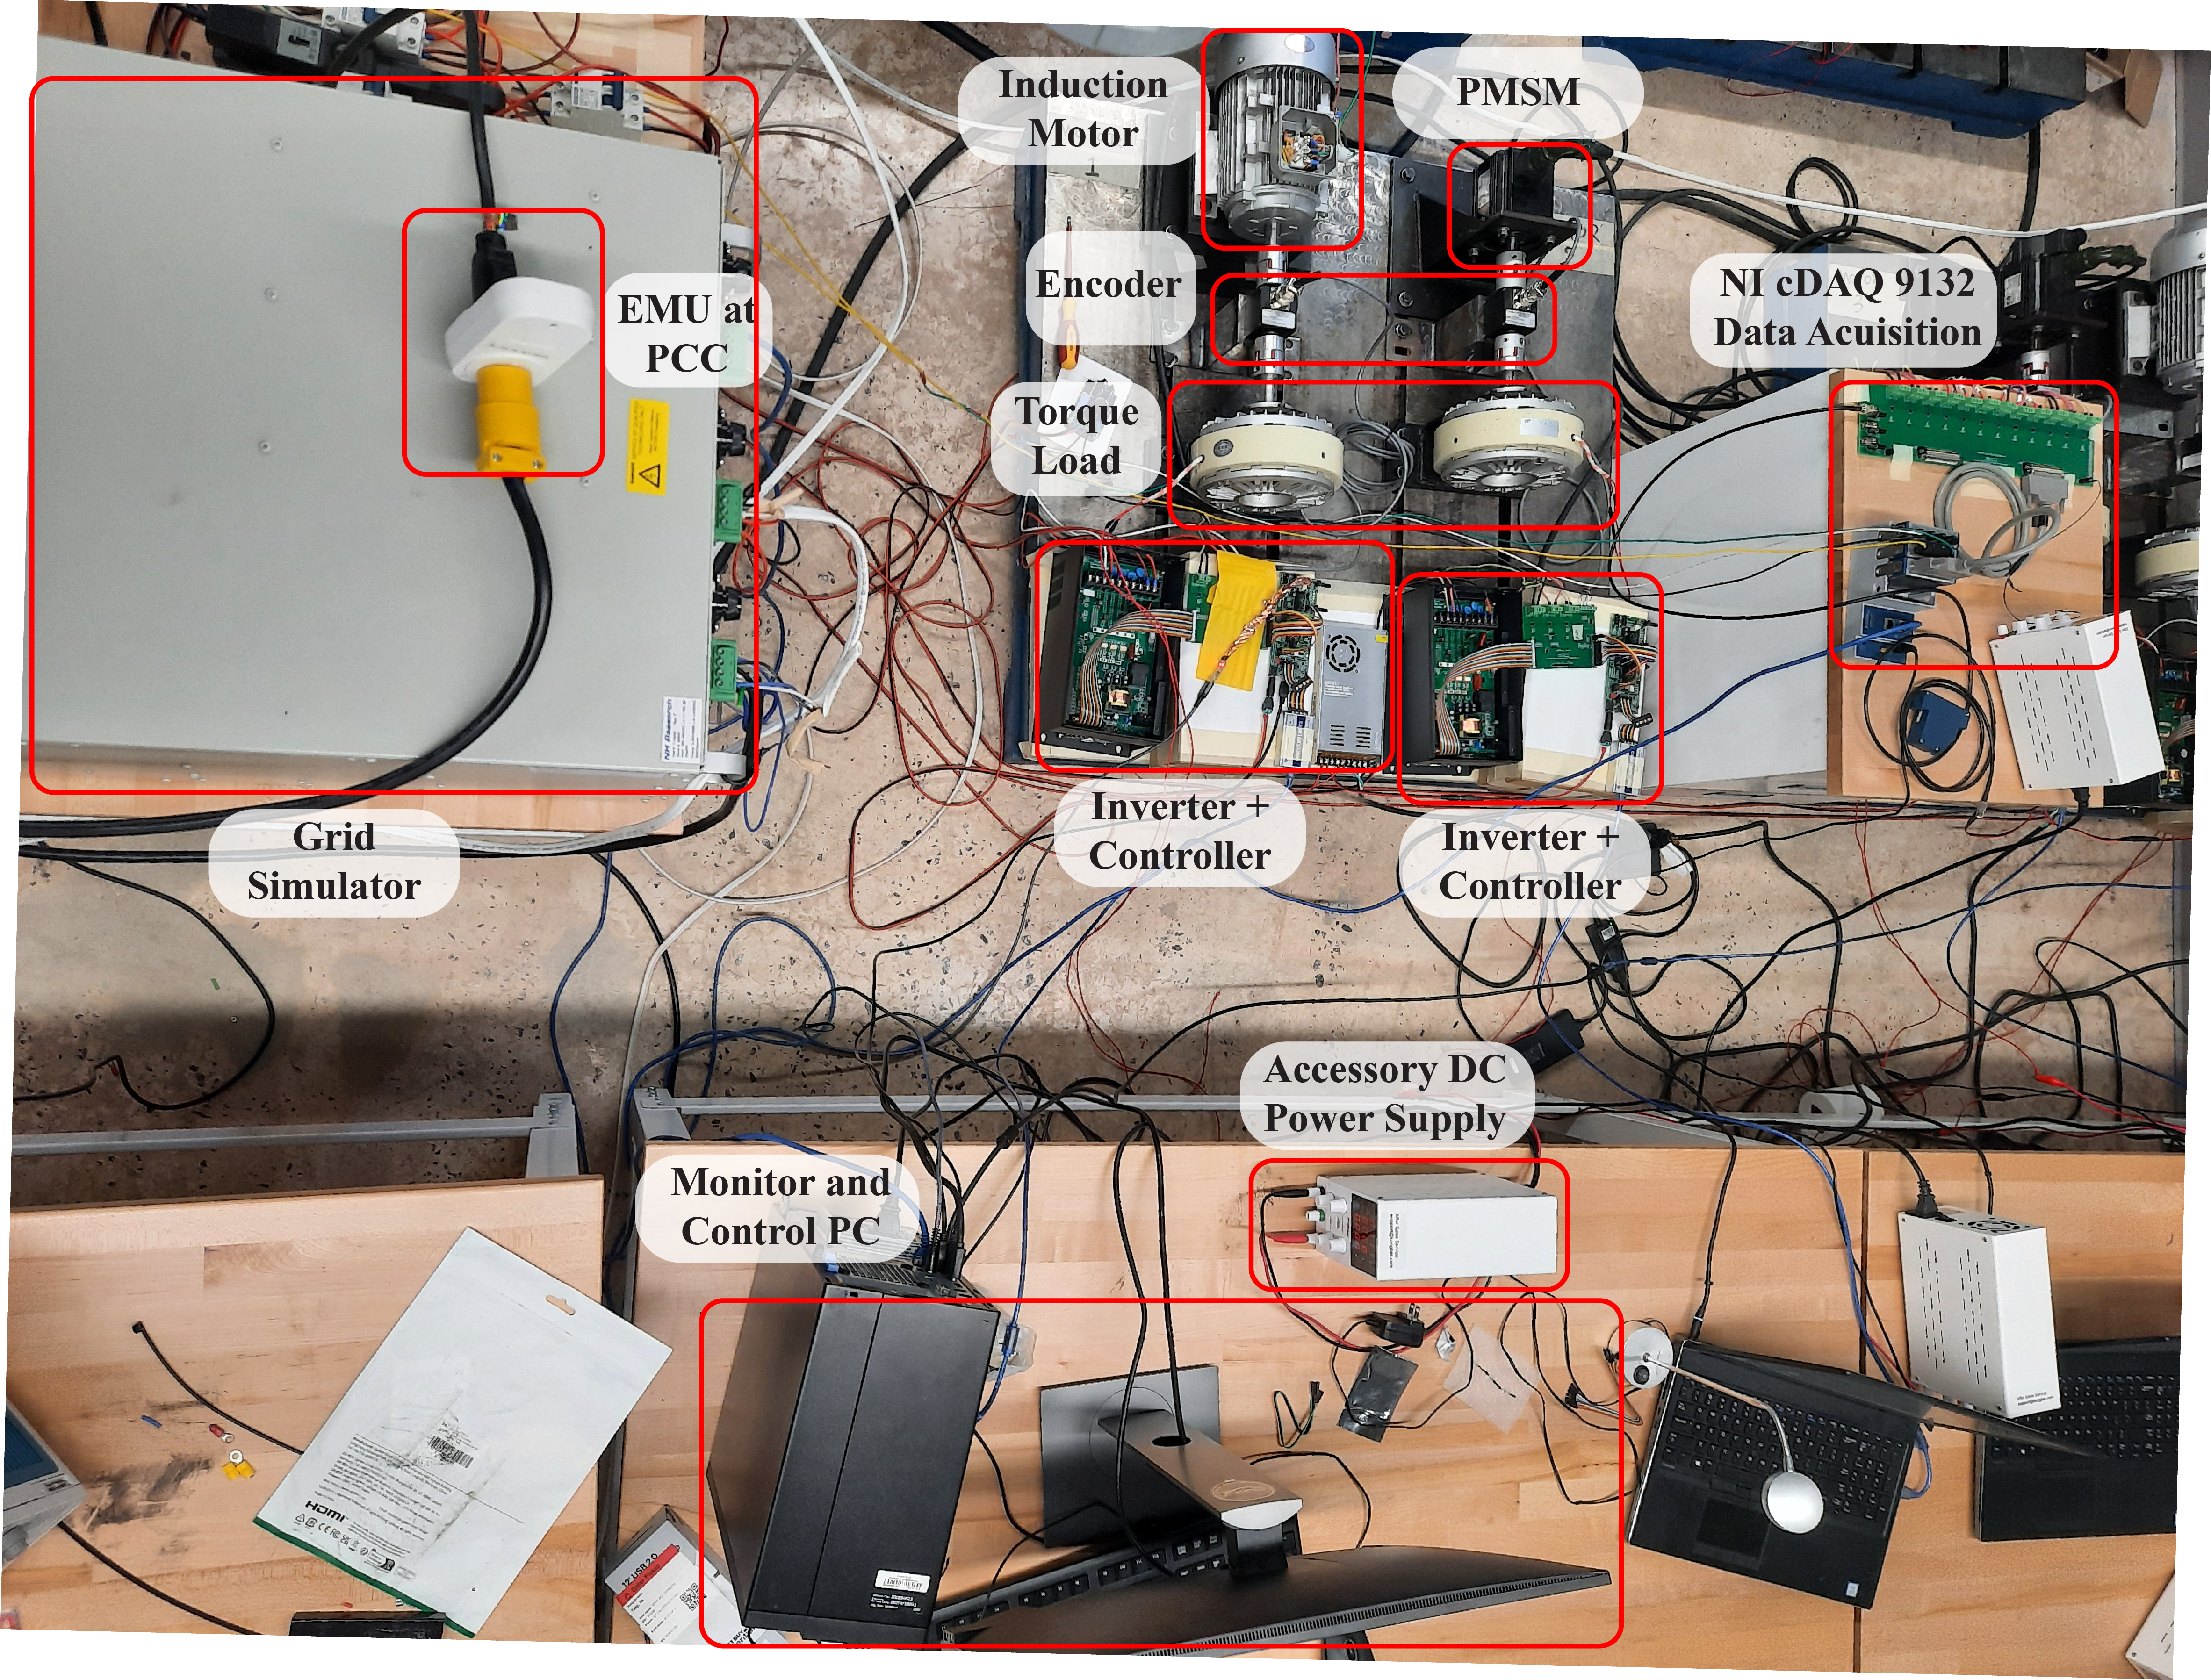
\includegraphics[width=0.5\linewidth]{figures/testbed[24].png}
    \caption{Physical Implementation of Power Flow}
\end{figure}
To safely emulate cyber incidents, false data injection attacks (FDIAs) are executed through pre-embedded firmware routines that introduce an offset-style bias injection on phase-current feedback signals. The attack model is defined as:
\begin{equation}
\tilde{\mathbf{i}}_{abc}(t) = \mathbf{i}_{abc}(t) + \boldsymbol{\alpha},
\end{equation}
where $\mathbf{i}_{abc}(t)$ is the true three-phase current vector and $\boldsymbol{\alpha}$ is the injected per-unit bias (applied per phase). Trials vary operating conditions (speed and load) and injection configurations (single-phase, two-phase, and multi-point), with attack magnitudes swept over $\alpha \in \{0.00025,\ldots,0.00500\}$ pu. Each run includes steady-state operation, attack activation, and recovery, enabling scalable supervised labeling.

\subsection{Dataset Structure}
Add stride 16, the exact 16 features, the binary-label rule, metadata fields, and the dataset-schema table.
The continuous PCC time-series is segmented using an overlapping sliding window with length 128 time steps and stride 16. Each sample is represented as $X \in \mathbb{R}^{128 \times 16}$, where the 16 EMU features summarize voltage and current measurements (e.g., amplitude, phase, RMS, and THD). 

For binary detection, each window is assigned a label $y \in \{0,1\}$ derived from an \texttt{is\_attack} indicator. In addition, the dataset includes structured metadata for richer analyses, including attack onset index within the window, motor type (ACIM/PMSM), phase targeting, severity level(s), and operating-point context (speed/load). This structure supports both real-time binary detection and future multi-class or condition-aware studies. 

Table.~\ref{tab:dataset_schema} summarizes the input feature groups used to construct X and the associated output labels and contextual metadata used in the dataset.
The learning task is to estimate $\hat{y}=f_{\theta}(X)$ from these labeled windows, providing a benchmark for detecting stealthy cyber-physical anomalies.

\begin{figure}[htpb]
    \centering
    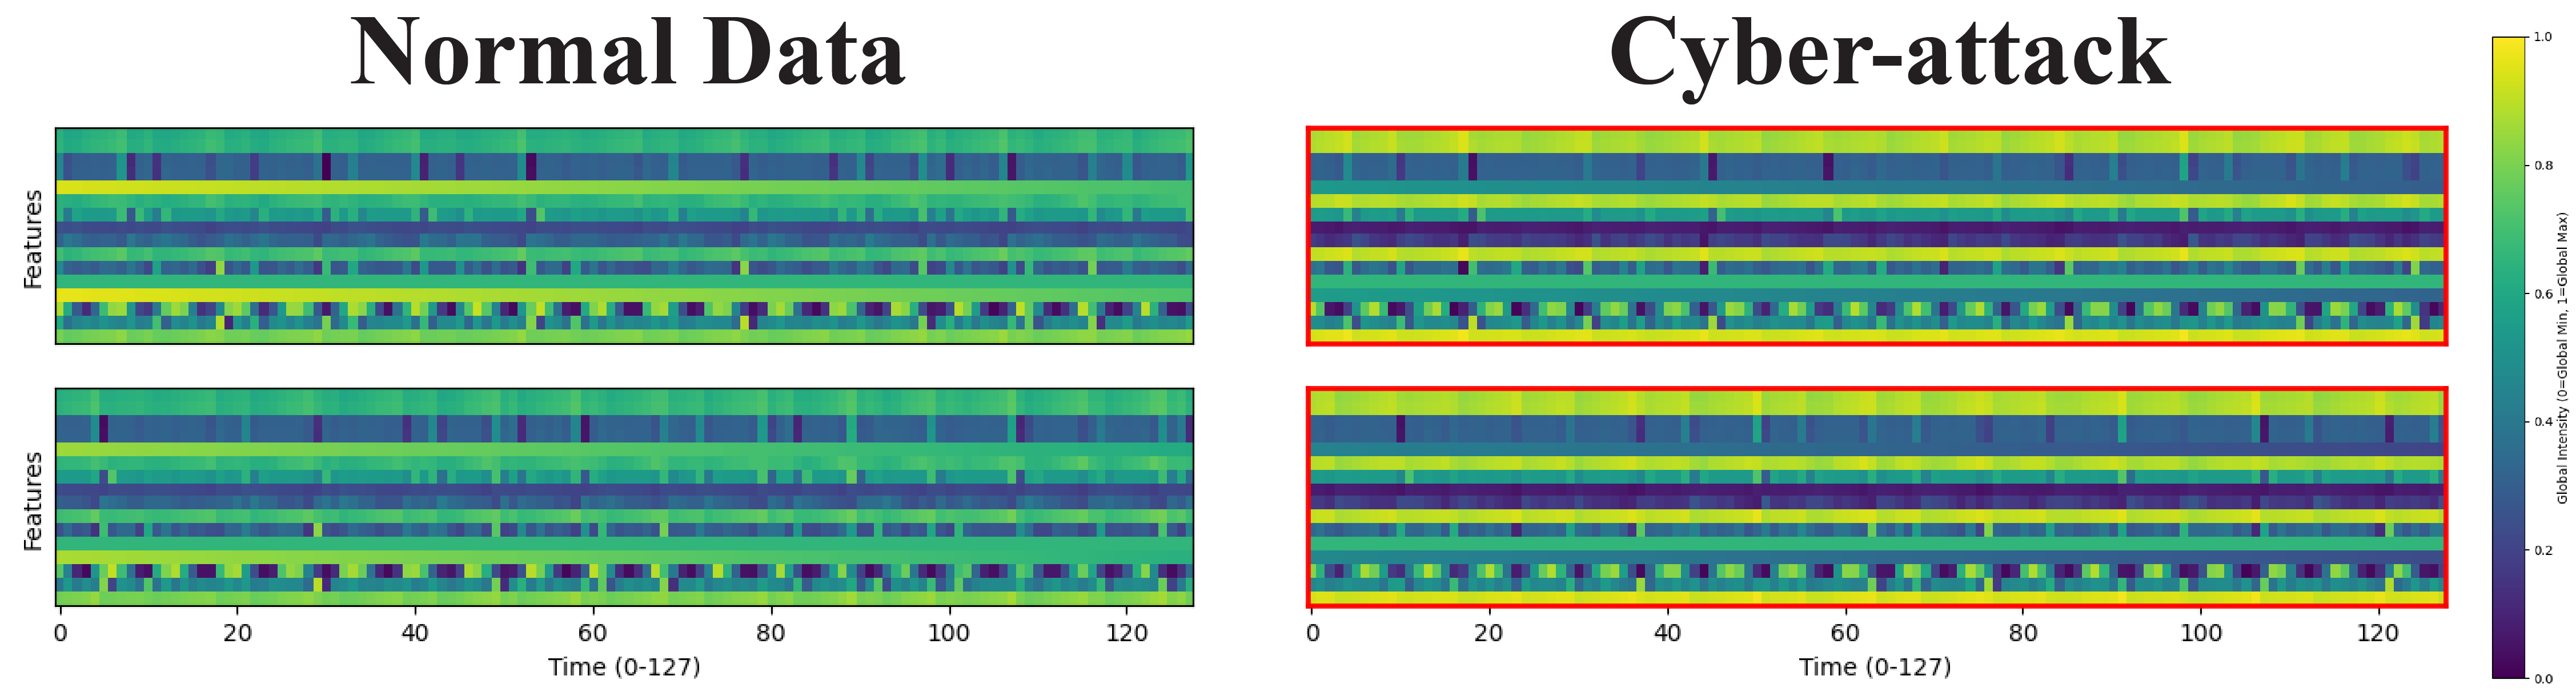
\includegraphics[width=1\linewidth]{figures/signals.png}
    \caption{Normal vs Cyber-attack data}
\end{figure}
The label vector \texttt{y} provides extensive metadata to support both binary and multi-class research objectives. Its 13 columns include flags for \texttt{is\_attack} (set to 1 if any sample in the window is an attack), \texttt{is\_onset} (the index of the first attack sample in the window), \texttt{attack\_id}, \texttt{attack\_type}, and the targeted \texttt{Motor} (encoded as 1 for ACIM, 2 for PMSM, and 0 for None). Additional columns detail the specific phase targeted (A, B, C), the corresponding severity levels, and any speed or load alterations. This comprehensive labeling logic relies on max-pooling the metadata over the duration of the window.

\begin{table}[H]
\centering
\caption{Dataset Input ($X$) and Label ($y$) Schema}
\label{tab:dataset_schema}
\begin{tabular}{l|l|c}
\hline
\textbf{Input (X)} & \textbf{Features} & \textbf{Count} \\ \hline
Current Features & Amp, Amp$_2^*$, Freq, Freq$_2^*$, Phase, RMS, ROCOF, THD & 8 \\
Voltage Features & Amp, Amp$_2$, Freq, Freq$_2$, Phase, RMS, ROCOF, THD & 8 \\ \hline
\textbf{Output (y)} & \textbf{Description} & \textbf{Scope} \\ 
\hline
\texttt{is\_attack} & Binary (0=Normal, 1=Attack) & 2 \\
\texttt{is\_onset} & First attack index in window (0--127) & 128 \\
\texttt{attack\_type} & Attack mode (normal:0, cyber\_attack:1) & 2 \\
\texttt{Motor} & 0=None, 1=ACIM, 2=PMSM & 3 \\
\texttt{A, B, C} & Phase-specific injection flags (0 and 1) & 2 \\
$\text{sev}_A, \text{sev}_B, \text{sev}_C$ & Intensity per phase (0.00025, 0.00050, \ldots, 0.00500) & 20 \\
\texttt{speed} & Motor speed settings (700, 1000, and 1300 RPM) & 3 \\
\texttt{load} & Motor torque load settings (2, 3, and 4) & 3 \\
\texttt{attack\_id} & Unique event identifier & 2730 \\ \hline
\multicolumn{3}{l}{$^*$Amp$_2$ and Freq$_2$ denote the second dominant amplitude and frequency components.} \\
\end{tabular}
\end{table}

\begin{figure}[h]
    \centering
    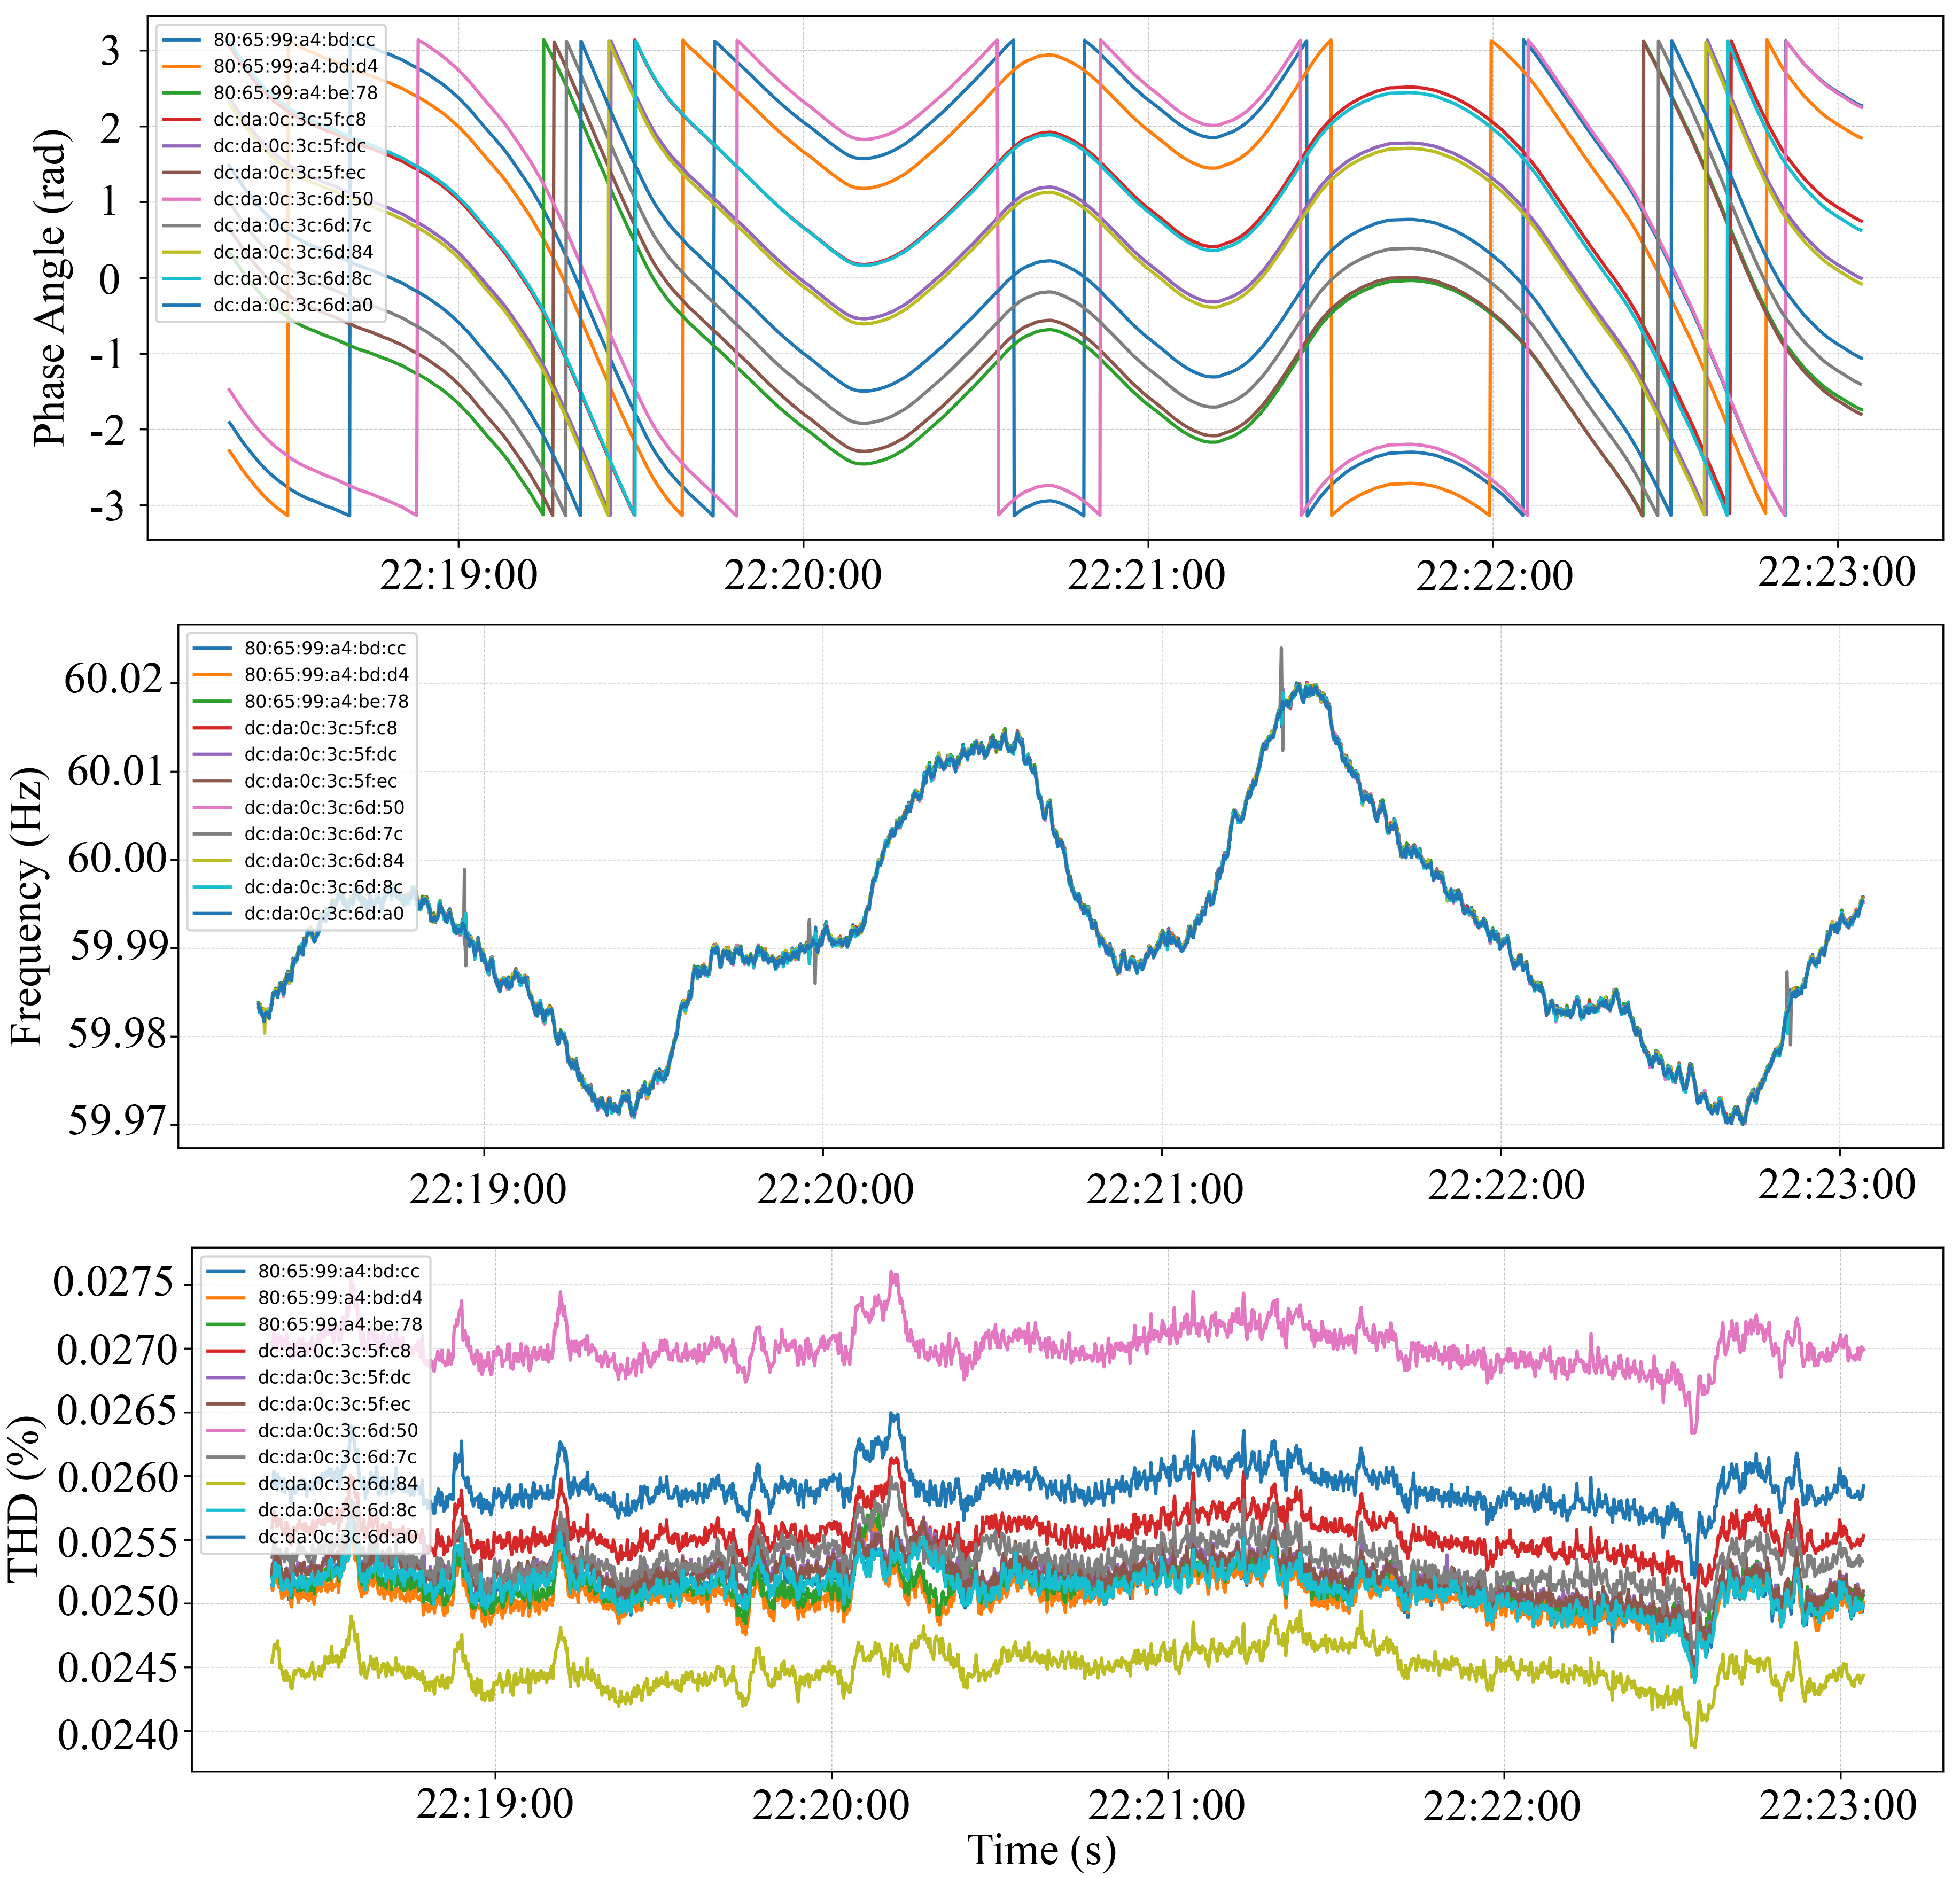
\includegraphics[width=0.5\linewidth]{featurescombined.png}
    \caption{Comparative time-series visualization distinguishing normal operational baseline sequences from injected cyber anomalies.}
\end{figure}

\section{Bidirectional GRU Architecture}

Recurrent models are well-suited for EMU time-series classification because cyber anomalies often manifest as subtle temporal deviations rather than isolated point events. We initially evaluated an LSTM baseline, but adopted a Bidirectional GRU (Bi-GRU) to reduce gating complexity while capturing contextual dependencies across each observation window.

Prior to training, each EMU sample is a fixed-length sequence. We augment each window by concatenating first-order temporal differences along the feature axis (from $128\times16$ to $128\times32$), followed by feature-wise standardization using statistics from the training split. The overall data acquisition, preprocessing, and model inference pipeline is illustrated in Fig.~\ref{architecture}.
The classifier comprises two Conv1D blocks (64 filters, kernel size 3) with Batch Normalization, followed by a Bidirectional GRU for sequence modeling. Outputs are aggregated with GlobalAveragePooling1D, passed through a 64-unit dense layer with 30\% dropout, and mapped to a sigmoid node for binary classification.
\begin{figure}[H]
    \centering
    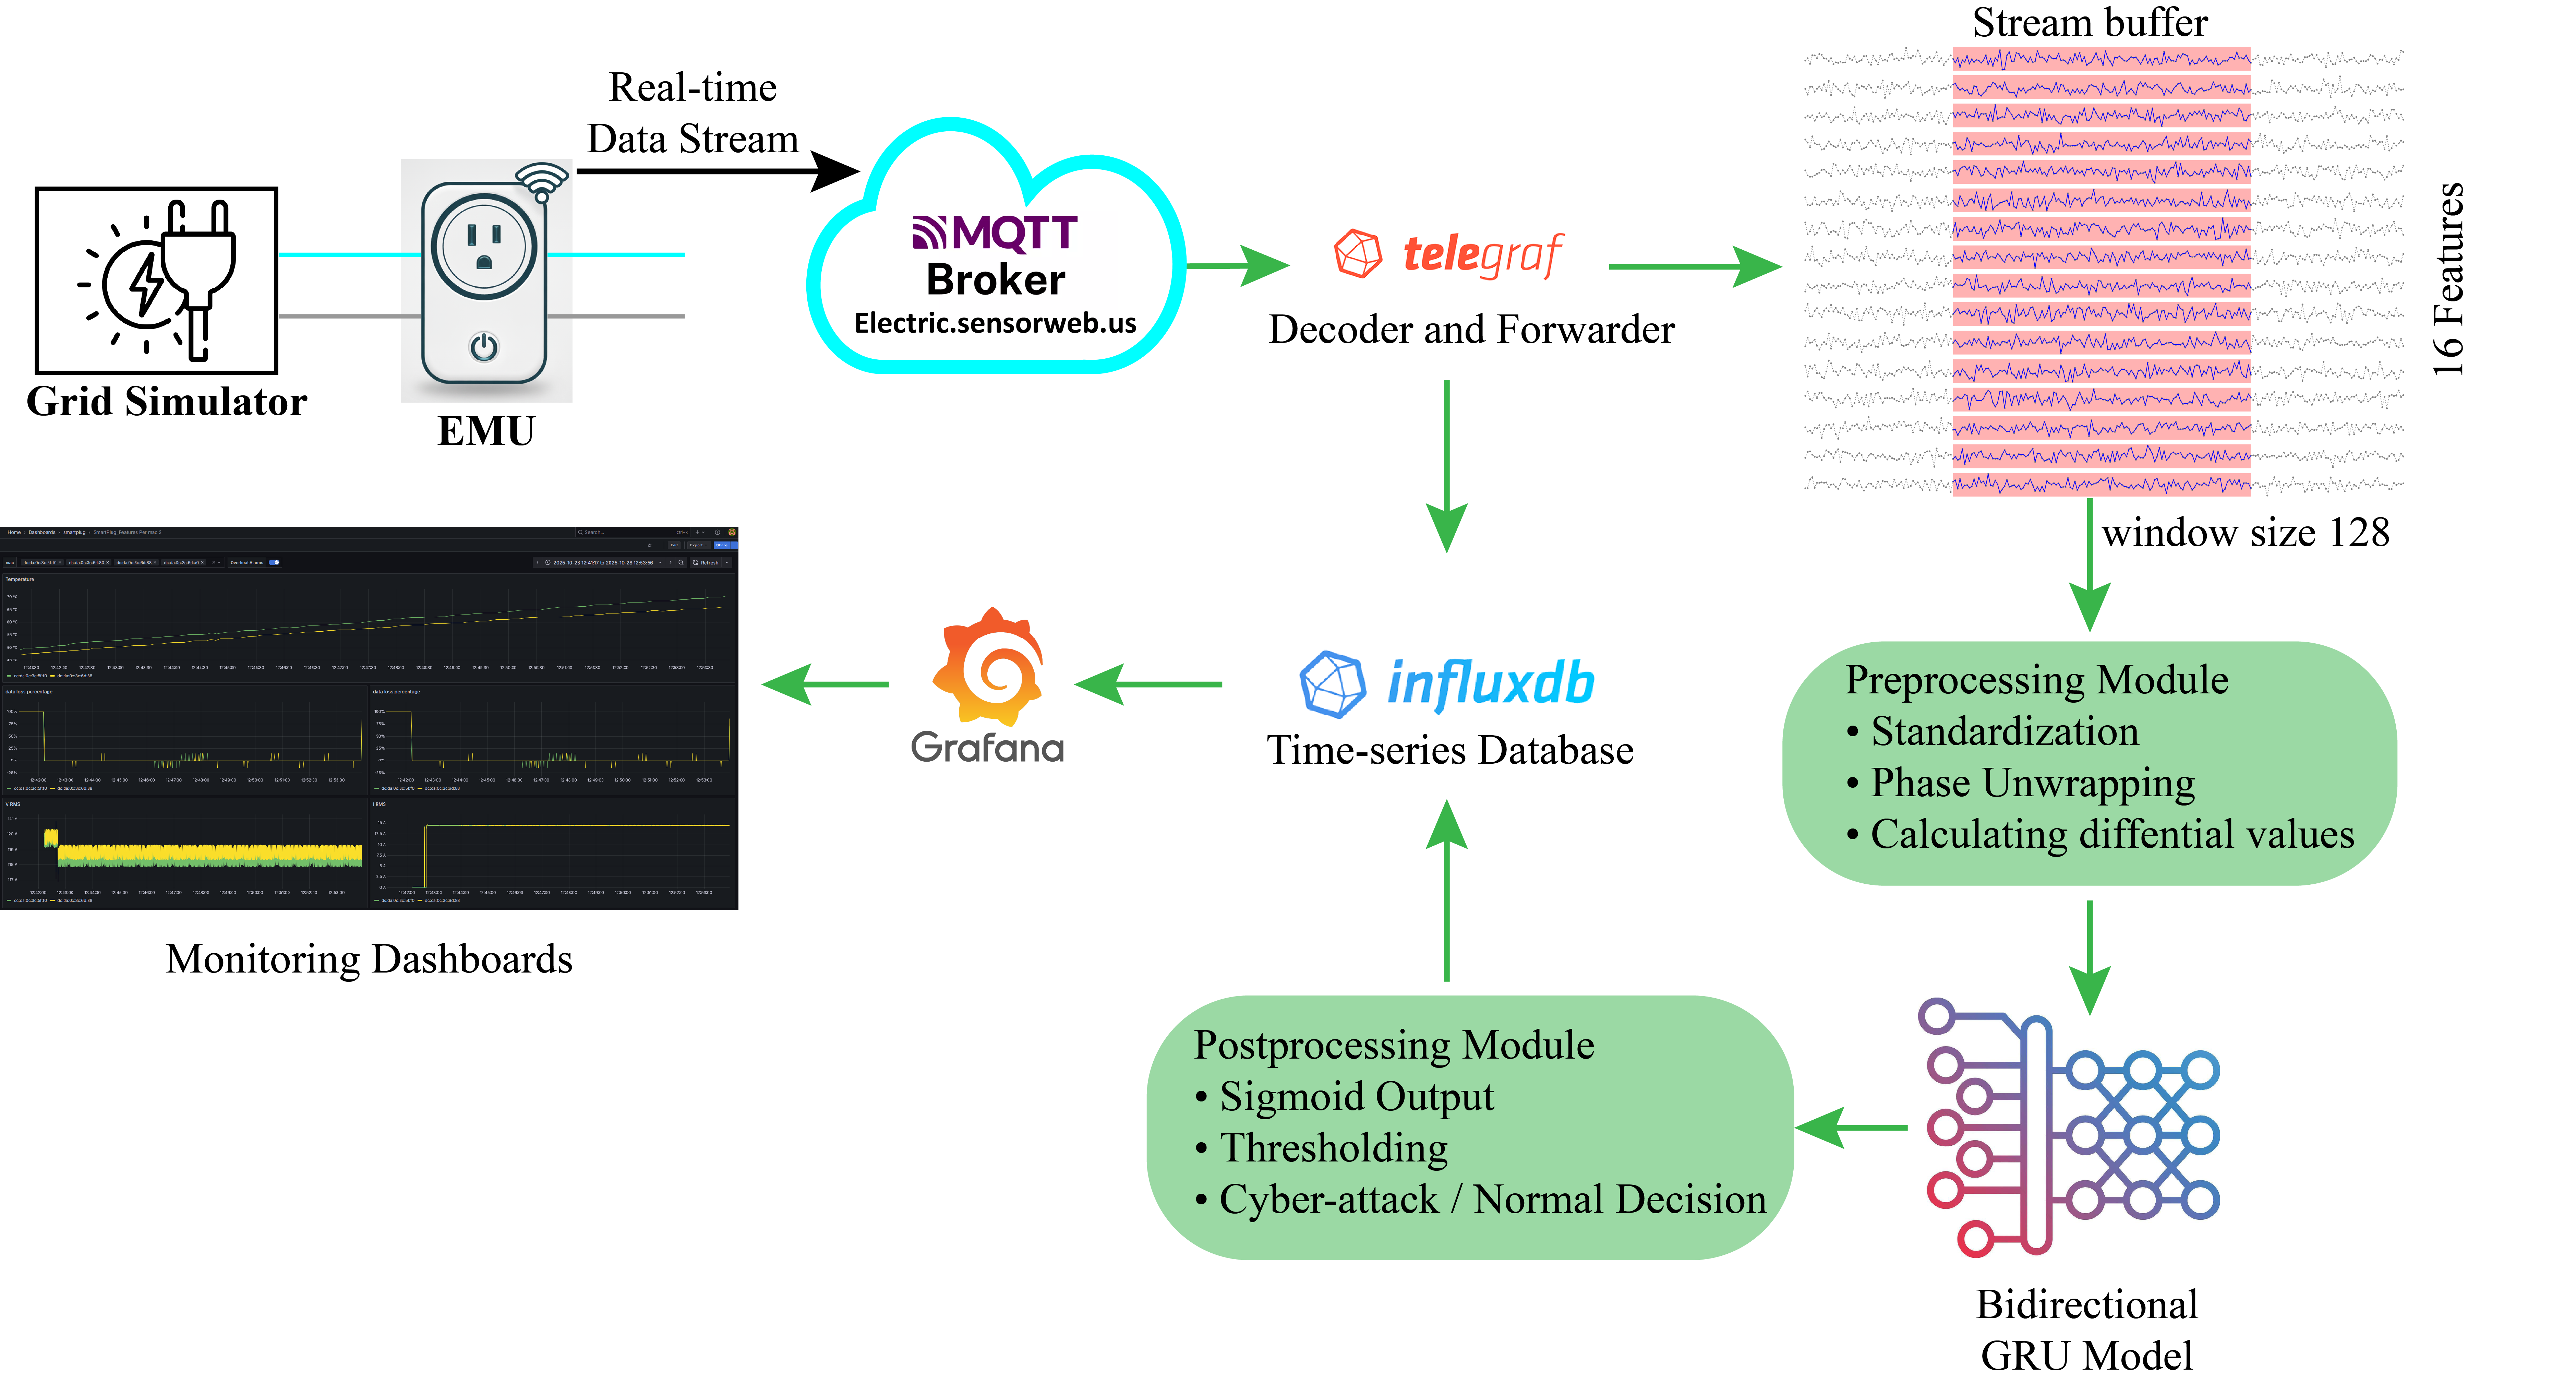
\includegraphics[width=0.7\linewidth]{figures/schematic diagram.png}
    \caption{Information flow architecture detailing the dual-stream feature engineering and preprocessing pipeline.}
    \label{architecture}
\end{figure}


Regularization is provided by Batch Normalization, dropout, early stopping based on validation PR-AUC, and a cosine learning-rate schedule.

\subsection{Addressing Class Imbalance}
The merged dataset is class-imbalanced (roughly 80\% attack and 20\% normal). Rather than rebalancing through under/oversampling, the full dataset is retained and split using stratified train-test partitioning to preserve the original class proportions. Imbalance is handled during optimization via class-weighted binary cross-entropy, with fixed weights (\texttt{normal}=1.0, \texttt{attack}=1.5). This increases the cost of attack misclassification while preserving complete coverage of normal operating behavior.

\subsection{Temporal Feature Engineering}
Early iterations used only first-order differences to emphasize signal velocity; however, this removed absolute magnitude information. The final pipeline computes first-order differences, preserves sequence length by prepending the first time step, and concatenates the differences with the raw features. The resulting representation is feature-wise standardized, providing both absolute-state context and rate-of-change dynamics.

\section{Experimental Results and Threshold Tuning}

The network is trained with Adam and binary cross-entropy. Because cyber-attack detection prioritizes missed-attack reduction, performance is tracked using Precision, Recall, and PR-AUC rather than accuracy alone.

%Training uses a cosine learning-rate schedule (decaying to 10\% of the base rate) and early stopping on validation PR-AUC with best-weight restoration. 
To improve the operating point beyond the default sigmoid threshold, we apply an epoch-wise threshold tuning routine that scans decision thresholds in $[0.1,0.9]$ and selects the value maximizing validation F1. With class-weighted training, dual-stream (raw+differential) inputs, and the Bi-GRU architecture, the proposed pipeline substantially outperforms the LSTM baseline and achieves $\sim$92\% test accuracy. It remains effective for low-severity attacks, achieving $\sim$96\% detection accuracy for $(0<\alpha \le 0.001)$ (Fig.~\ref{fig:Severityeffect}).

To contextualize these results, we compare against an unoptimized LSTM baseline and prior PMU-based \cite{guha} and IED-based \cite{aljohani2024} approaches, as summarized in Table.~\ref{tab:comparison} While these infrastructures can reach comparable accuracies, they require higher-cost instrumentation and are less suitable for consumer-edge deployment. In contrast, our EMU-based Bi-GRU framework provides competitive performance using low-cost sensing at the PCC.
\begin{figure}
    \centering
    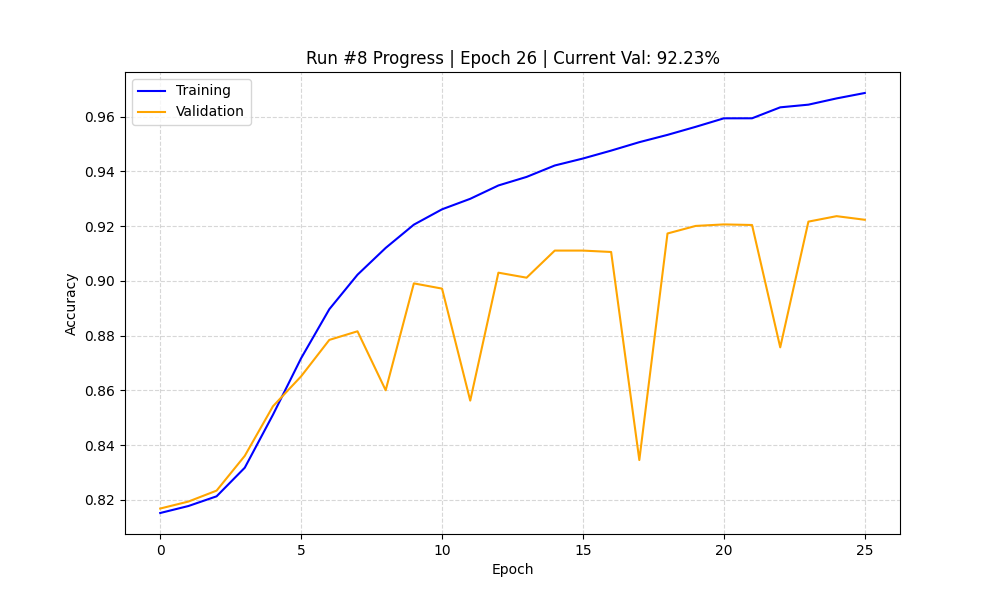
\includegraphics[width=0.5\linewidth]{image.png}
    \caption{Training and Validation Accuracy over Epochs}
    \label{fig:placeholder}
\end{figure}

\begin{table}[H]
    \centering
    \caption{Performance Comparison with Existing Cyber Anomaly Detection Schemes}
    \label{tab:comparison}
    \renewcommand{\arraystretch}{1.3} % Adds a little padding to the rows
    \begin{tabular}{|l|c|c|c|c|}
        \hline
        \textbf{Methodology} & \textbf{Sensor Data} & \textbf{Accuracy} & \textbf{Real-Time} & \textbf{Edge Scalability} \\
        \hline
        Aljohani \textit{et al.} \cite{aljohani2024} (LSTM) & IED / Substation & $\sim$95\% & Yes & Low (High Cost) \\
        \hline
        Guha \textit{et al.} \cite{guha} (VAE) & PMU & $\sim$89\% & No & Low (High Cost) \\
        \hline
        Initial Baseline (Standard LSTM) & EMU & $\sim$81\% & Yes & High (Low Cost) \\
        \hline
        \textbf{Proposed (Bi-GRU)} & \textbf{EMU} & \textbf{$\sim$92\%} & \textbf{Yes} & \textbf{High (Low Cost)} \\
        \hline
    \end{tabular}
\end{table}

\begin{figure}
    \centering
    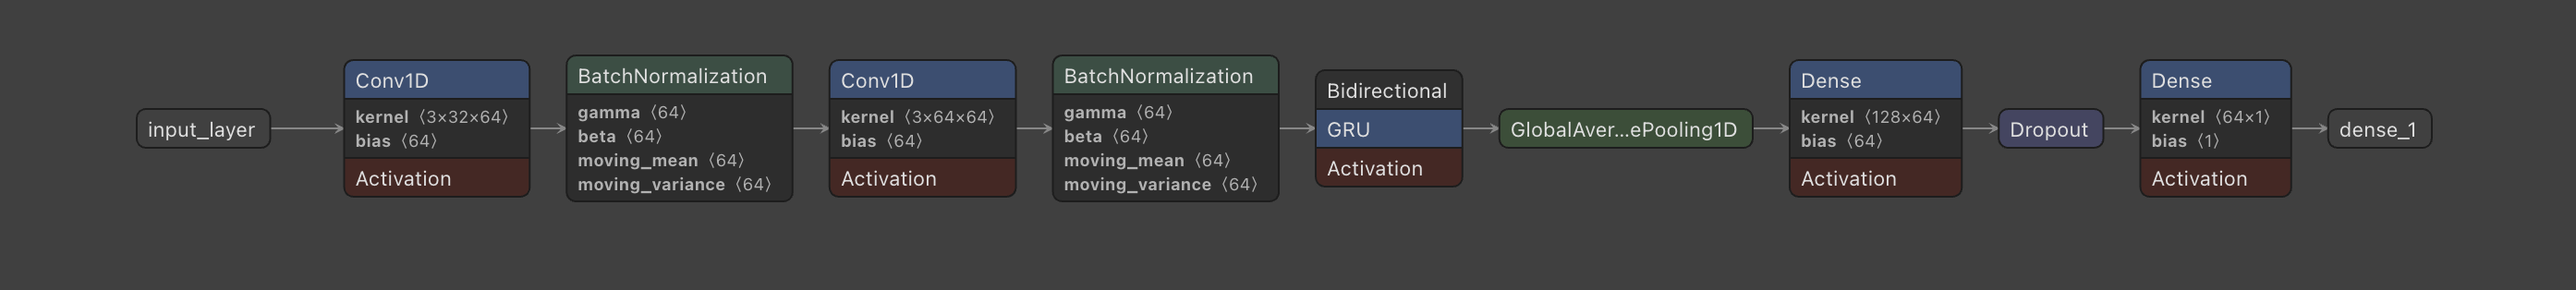
\includegraphics[width=1\linewidth]{Screenshot 2026-03-06 at 10.53.36 PM.png}
    \caption{Model Structure}
    \label{fig:placeholder}
\end{figure}

\clearpage
\begin{figure}
    \centering
    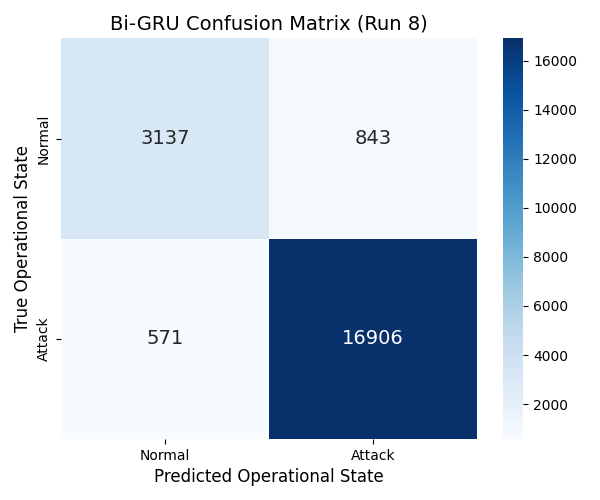
\includegraphics[width=0.5\linewidth]{Confusion}
    \caption{Confusion Matrix}
    \label{fig:placeholder}
\end{figure}

\begin{figure} [H]
    \centering
    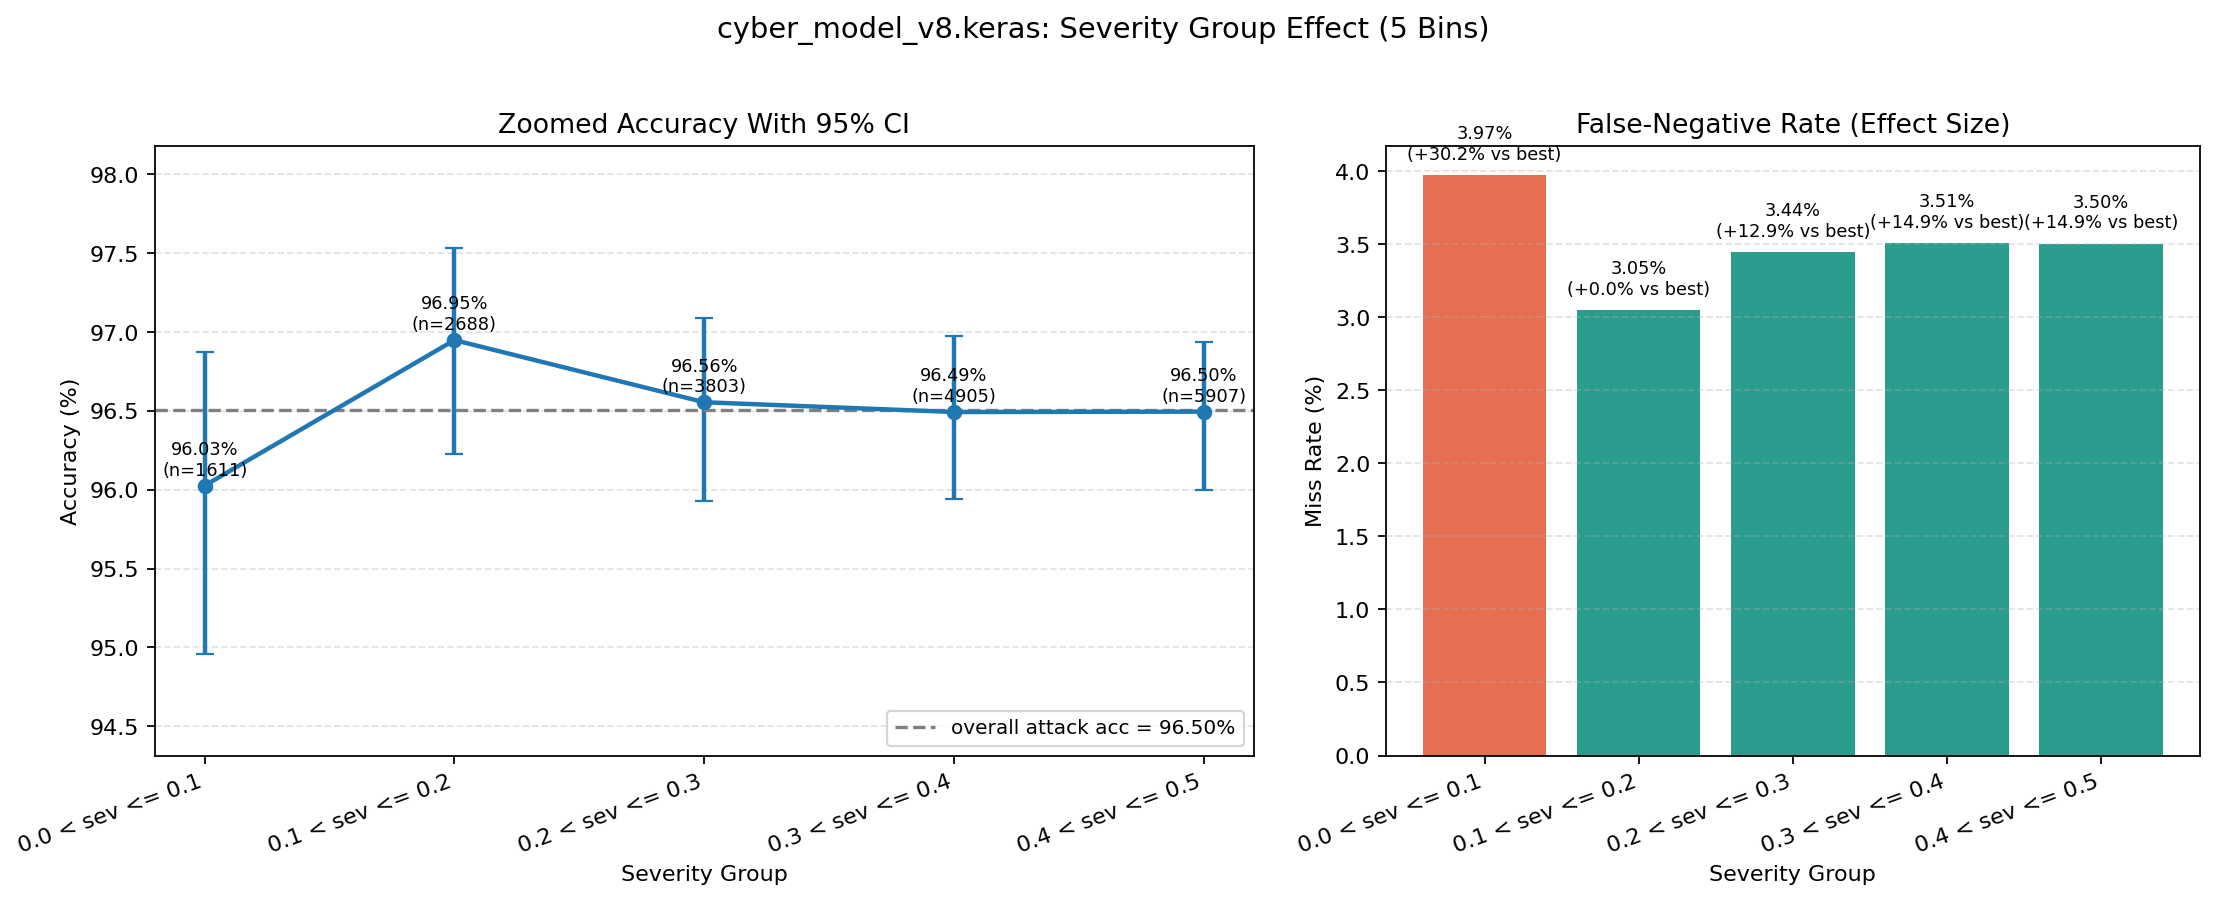
\includegraphics[width=\textwidth]{figures/plot_severity_group_effect_5bins.png}
    \caption{Accuracy and False Negative in Different Severity Groups}
    \label{fig:Severityeffect}
\end{figure}


\section{Conclusion and Future Work}

This work successfully demonstrates that low-cost, IoT-enabled EMU can serve as highly effective, localized sensors for cyber attack detection in AC power systems. By addressing critical data bottlenecks through class weighting and advanced feature preservation, the proposed Bidirectional GRU framework reliably processes complex 16-feature time-series data to classify operational states with high accuracy. Having established this supervised benchmark, future work will expand the framework to detect a broader range of fault and disturbance scenarios beyond cyber attacks (e.g., abnormal operating conditions and component-level faults). We will also extend the PCC-based measurement strategy to function as a comprehensive observability layer, enabling unified monitoring and event classification using EMU data at the PCC.

\bibliographystyle{IEEEtran}
\bibliography{IEEEabrv,bibliography}

\end{document}
